\chapter{Results and Discussion}

In this chapter I present and discuss the results of my work.
The first section, \cref{sec:long_waveguide}, presents the simulations needed to
ascertain that the beamsplitter simulations would work as intended.
This includes tuning the \gls{pml} parameters and checking that the excitation
excites the right mode.
After that, I present the results of the continuous optimization followed by the
results for the level-set optimization in \cref{sec:res_cont,sec:res_bin}
respectively.
In summary, the continuous optimization yielded near perfect devices with full
transmission and very little reflection.
The level-set optimizations never reached quite as good performance, with around
10\% of the power getting reflected.
\todoblk{BUT IT IS STILL INCREASING!}
% The continuous optimization efforts was plagued by a persistent failure to
% converge, and thus a large part of my work was to try to solve this.
% This failure to converge prevented a gradual shift toward binary devices,
% which would have allowed for a smoother transition to the
% level-set design paradigm.
% Nevertheless, the level-set methods were also tried,
% but with either manually set starting points or suboptimal designs seen in the
% continuous optimization.
% Finally, the continuous optimization did converge and yielded devices which
% transmitted approximately 95 \% of the incoming waves.

\section{Long waveguide simulations}\label{sec:long_waveguide}

As detailed in \cref{sec:methods}, a long waveguide without any beamsplitter
elements was simulated to ascertain that the excitation method correctly excited
only the desired mode, and that the \gls{pml} elements were reflectionless.
In this section I present the results from those simulations.
The waveguide used for these is pictured in \cref{fig:long_waveguide}

\begin{figure}[htpb]
	\centering
	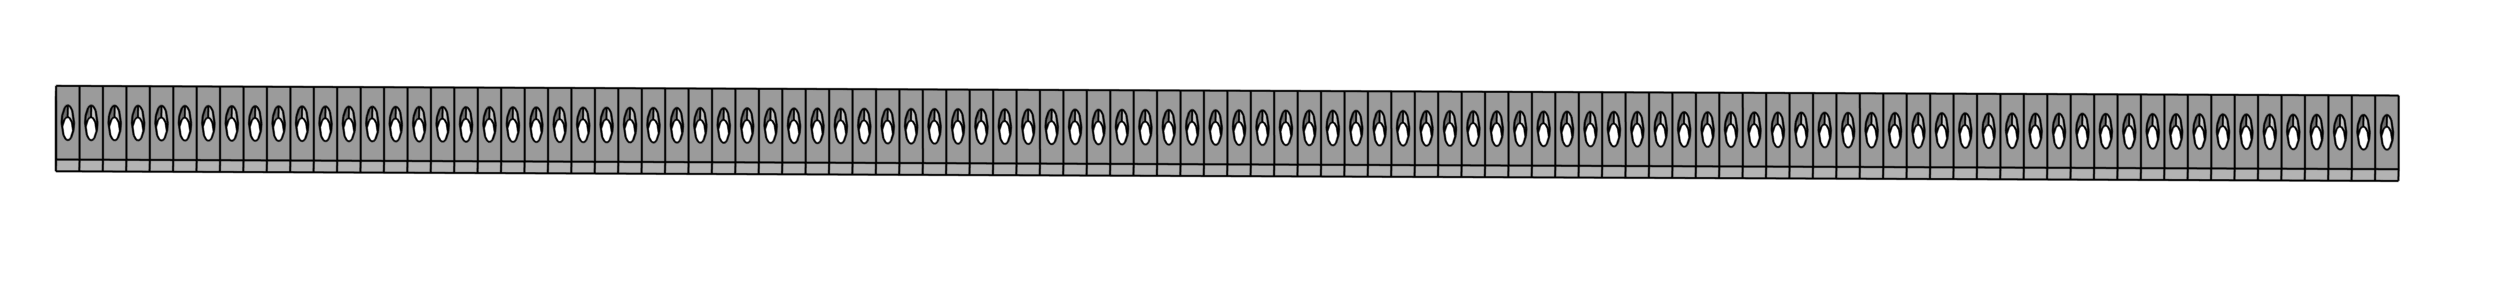
\includegraphics[width=\textwidth]{chapters/results/long_waveguide_geom.png}
	% 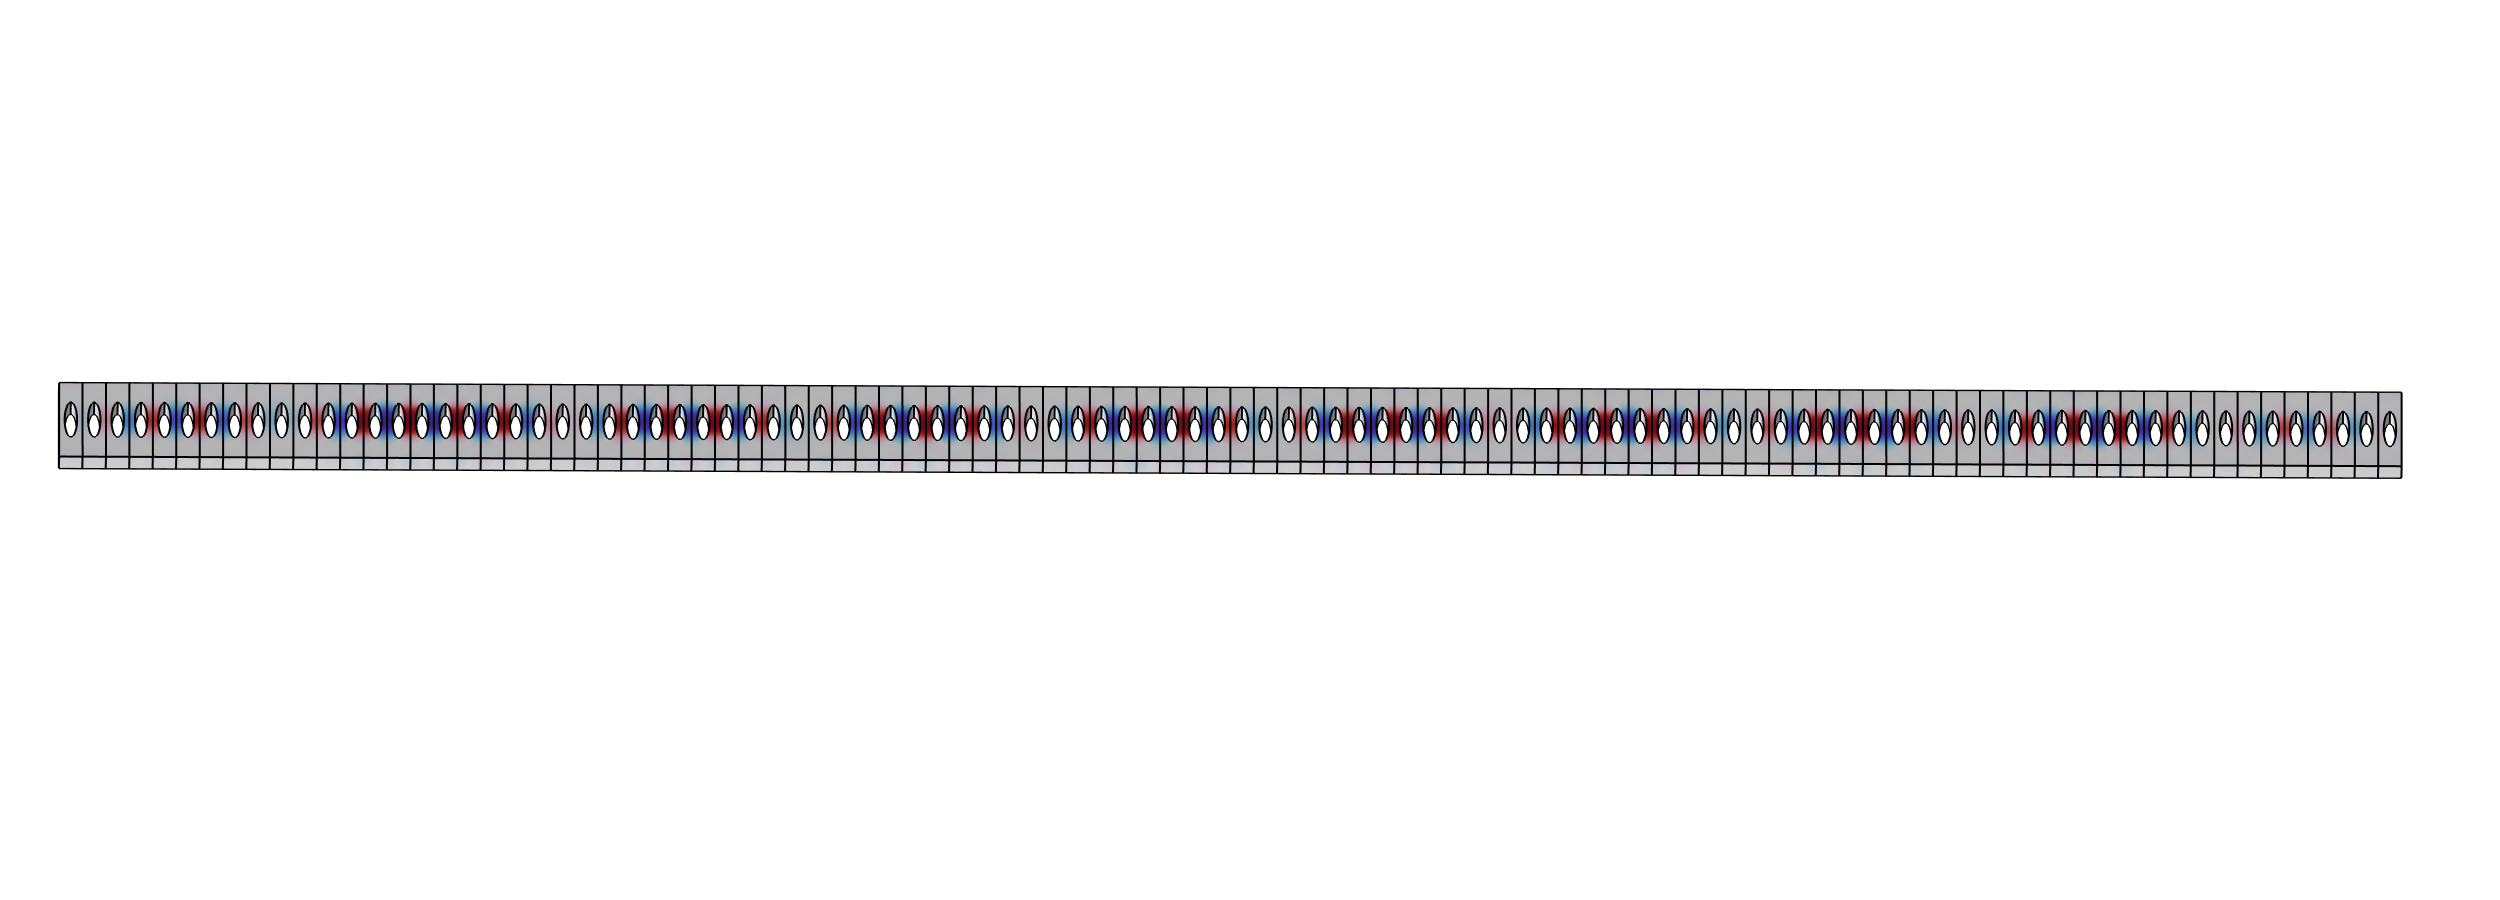
\includegraphics[width=\textwidth]{chapters/results/long_waveguide_v_d=5_s=0.02.png}
	% 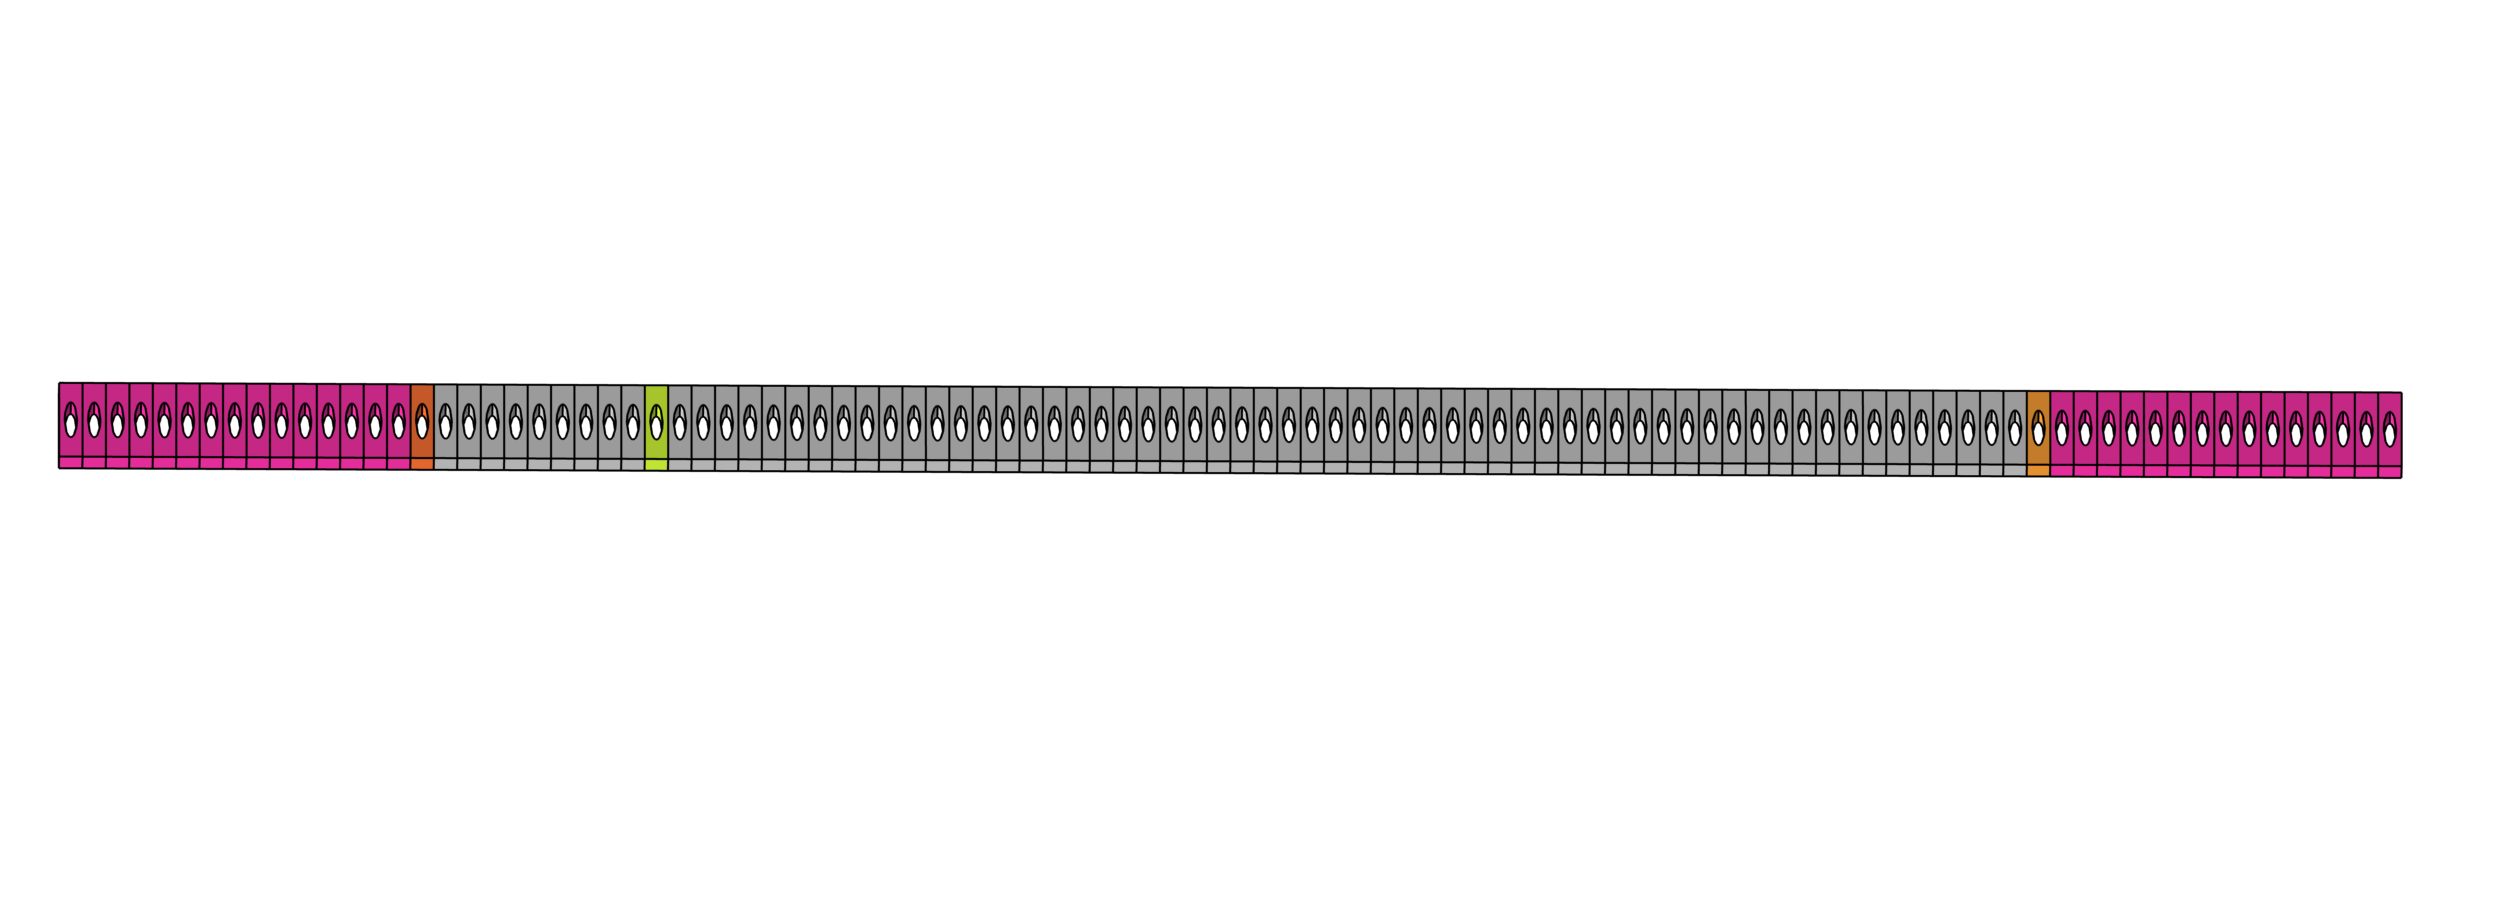
\includegraphics[width=\textwidth]{chapters/results/long_waveguide_selections.png}
	\caption{%
		This figure shows the long waveguide used for the \gls{pml} simulations
		as wells as validating the excitation method.
	}%
	\label{fig:long_waveguide}
\end{figure}

\subsection{Excitation}

The fact that the excitation was almost solely in the desired mode was verified
in two ways.
Firstly, as detailed in \cref{sec:excitation_method}, $a$ and $b$ in $u = a u_m
+ b u_r$ was computed.
The result was that $a = 1.166$ and $b = 0.0327$.
Thus $99.92\%$ of the energy was in the desired mode.
Secondly, a fourier transform of the y-component of the displacement field was
made.
This can be seen in \cref{fig:v_ft}.
The other modes that could be excited at this frequency have very different wave
vectors, which means that they would show up as separate peaks somewhere around
$0.4 \pi / a$ and $0.1 \pi / a$.
Since no other peaks can be seen, this further supports the result that only the
desired mode is excited.

\begin{figure}[htpb]
	\centering
	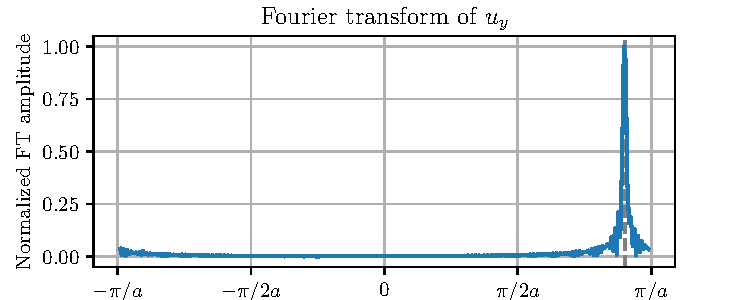
\includegraphics{chapters/results/ft_figure.pdf}
	\caption{%
		Fourier transform of the y-component of the displacement field.
		It clearly shows one wave traveling forward with a k-vector of
		$0.9 \pi / a$, where the dashed gray line is.
		Since the closest other mode at this frequency is at
		$k_y \approx 0.4 \pi / a$, where no peak is visible, it is concluded
		that solely the desired mode is excited.
	}%
	\label{fig:v_ft}
\end{figure}

\subsection{PML investigation}

\Cref{fig:pml_sweep1} shows the amplitude of the reflection,
quantified as the peak height relative to the forward propagating wave,
for different profiles.
These figures fit well with the three types of reflection mentioned previously.
The leftmost plot in \cref{fig:pml_sweep_sd} shows that all of the different
shapes yield reflections when the derivative at the beginning of the \gls{pml}
is around \num{3e-4}, which indicates that the reflections are dominated by
effects from the sudden start of the \gls{pml}.
On the other end, the increase in reflection amplitude come from
waves reaching the end of the \gls{pml} and getting reflected there.
The third type of reflection seems to only be noticeable for $d \leq 4$.
It is also worth noticing that with lower $d$, the plateau where neither of the
first two kinds of reflections are significant is broader.
Since $d=5$ was the lowest $d$ to show no signs of the third type of reflection,
that was chosen for the shape of the \gls{pml} profile.
After that, we investigated how short we could make the it while retaining
low reflections. \Cref{fig:pml_sweep_sn} shows $s$ sweeps for different $n$.
To achieve a short yet functional \gls{pml}, $d=5$, $s=0.03$ and $n=20$ was
chosen.
For $n=15$, reflections from the beginning start to become significant before
the reflections from the end have waned.

\begin{figure}[htpb]
	\centering
	\begin{subfigure}[]{0.99\textwidth}
	\begin{center}
		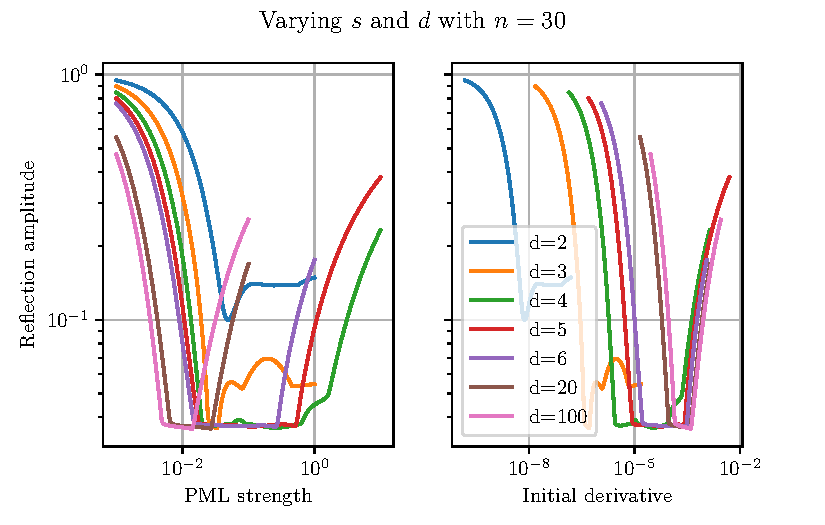
\includegraphics{chapters/results/pml_sweep_sd.pdf}
	\end{center}
	\caption{
		On the left is the reflection amplitude plotted as a function of the
		\gls{pml} strength $s$ for different $d$.
		For $d > 4$ there are two sources of reflection:
		for small $s$ reflection at the end of the \gls{pml} occurs,
		and for large $s$, there is reflection at the beginning.
		The right figure makes it clear that it is the slope at the beginning of
		the \gls{pml} that matters, since the point at which it becomes
		significant is the same for all $d$.
	}
	\label{fig:pml_sweep_sd}
	\end{subfigure}%

	\begin{subfigure}[]{0.99\textwidth}
	\begin{center}
		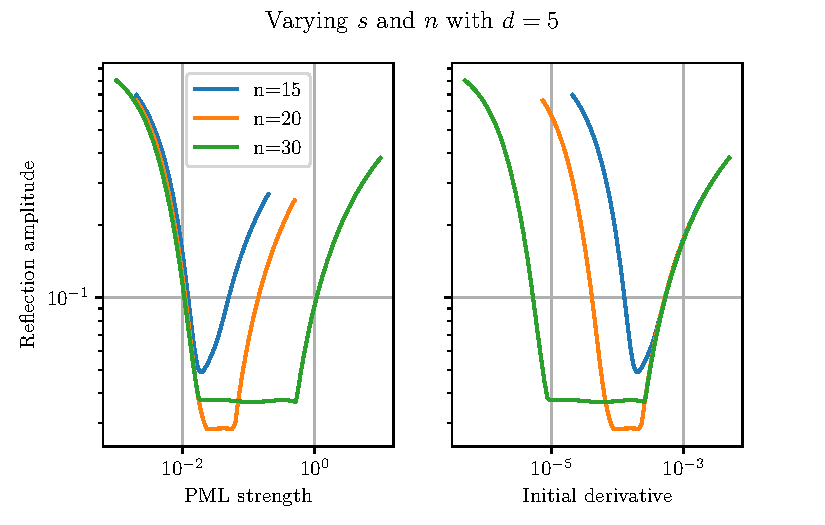
\includegraphics{chapters/results/pml_sweep_sn.pdf}
	\end{center}
	\caption{
		This is the same as \cref{fig:pml_sweep_sd} but with varying $n$.
		For $n=15$, the reflections from the beginning do not subside before the
		reflections from the end become significant, so at least $n=20$ is
		necessary.
	}
	\label{fig:pml_sweep_sn}
	\end{subfigure}
	\caption{}
	\label{fig:pml_sweep1}
\end{figure}

\section{Continuous optimization}\label{sec:res_cont}

There was a lot of problems with the optimization of the continuous design.
Many optimization runs would end up looking like \cref{fig:bad_cont_conv},
reaching a somewhat performant beamsplitter but invariably declining after some
point.
The figure shows the evolution of the transmitted power in one of the
output arms, as well as the reflected power back into the input.
This has been normalized such that 1 is the power in through the input waveguide.
Thus, an optimal beamsplitter would reach 0.5.
If the powers do not add up, it is because energy is flowing out in a different
mode.
I tested a few different theories on why the algorithm might fail to converge.
The first one was that perhaps the simulations were unstable for the case when
$p\approx 0$. To test this I interpolated between $\rho^\text{si}$ and
\qty{1000}{\kg\per\m^3} instead. However, convergence was still not reached.
The second was that maybe the meshing was too coarse to resolve the design
field properly. However, this was not the case as increasing the meshing did not
change the objective function more than a percent or so, so this wasn't the
cause either.
The last thing I thought of was that comsol was using quadratic shape functions
for the fields. This means that on each finite element of the mesh, the fields
are approximated with quadratic polynomials. Thus, if one computes any third
order spatial derivative, it will be 0 everywhere, and the second order
derivatives will not be very accurate.
In \cref{fig:quad_spline_sine} I show how quadratic splines can give a very good
approximation to a function, while still being a terrible approximation to its
second derivative.
Since I used second derivates in computing my gradient, that also wasn't very
reliable.
One way of solving this is to use higher order shape functions, however this
greatly increases the degrees of freedom, making the problem too computationally
expensive, at least with our hardware and geometry.
Another way is to make the mesh much finer, but this is also too computationally
expensive.
\begin{figure}[htpb]
	\centering
	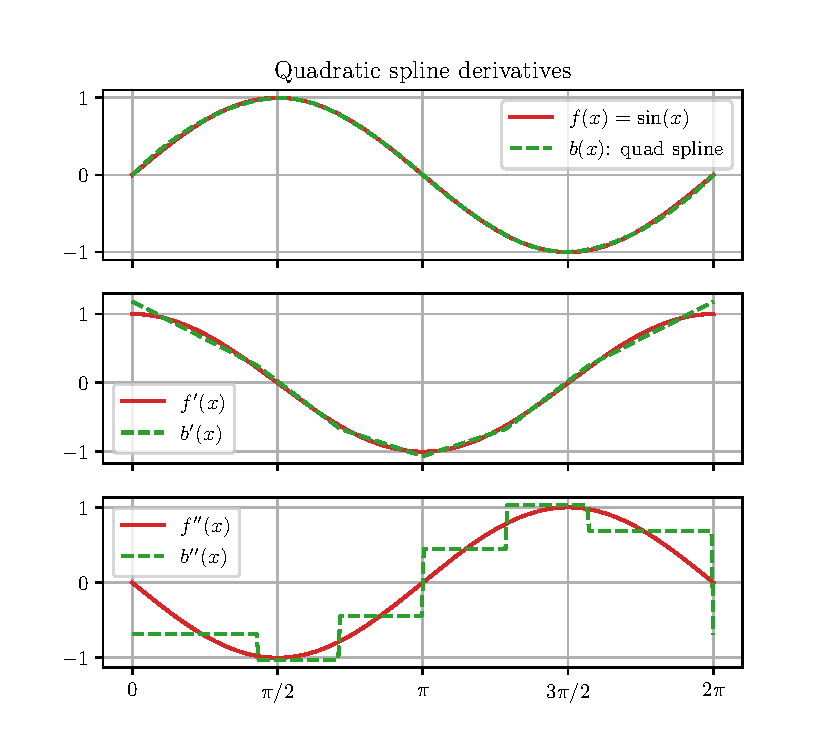
\includegraphics{chapters/results/quad_spline_sine.pdf}
	\caption{%
		This figure shows a quadratic spline approximation to a sine function,
		given eight points on the function. Even though the spline approximates
		the sine function very well, the second derivative approximation is
		terrible.
	}%
	\label{fig:quad_spline_sine}
\end{figure}

However, there was another way:
using the built in COMSOL function \mintinline{c}+fsens+ for computing
the gradient, convergence was obtained.
\Cref{fig:cont_conv1} shows the performance evolution of this optimization run.
At iteration 467, the model was deemed to have converged and as described in
\cref{sec:m_optimization}, a sigmoid function with $r=0.1$ was applied and optimization
continued.
At iteration 615, the model again seemed converged and $r$ was set to $0.05$.
Finally, at iteration 830, near perfect performance was reached and optimization
was terminated.
\Cref{fig:cont_design1} shows the design field after convergence for each of the
three stages.

\begin{figure}[htpb]
	\centering
	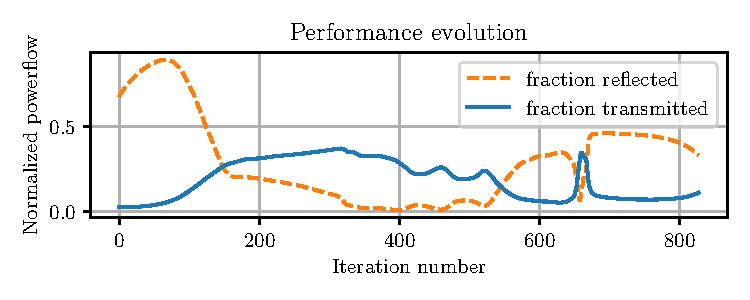
\includegraphics{chapters/results/conv_22.pdf}
	\caption{%
		Non-converging optimization example. The blue curve shows the
		transmitted power in one of the output arms as a function of iteration,
		while the yellow shows the power reflected back out through the input.
		The cases where two times the blue plus the yellow isn't 1.0 is
		explained by power exiting through a different mode.
	}%
	\label{fig:bad_cont_conv}
\end{figure}

\begin{figure}[htpb]
	\centering
	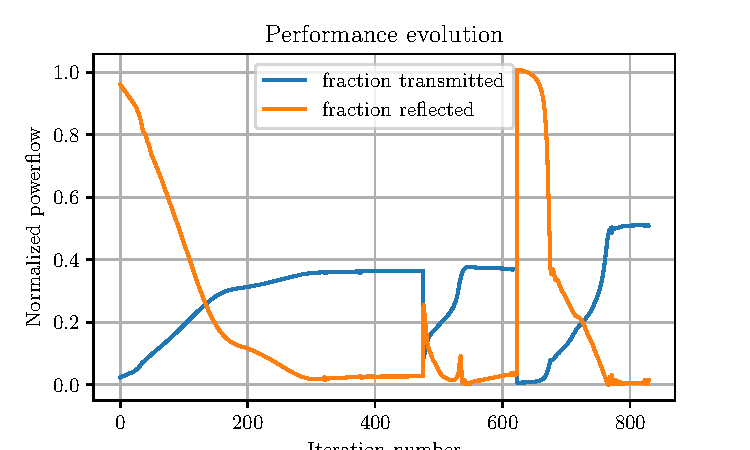
\includegraphics{chapters/results/conv_31.pdf}
	\caption{
		Similar to \cref{fig:bad_cont_conv},
		but at iteration 467 and 615, a sigmoid function was abruptly applied
		to the design field, which causes the dips.
		The final device was a near perfect beamsplitter, with less than 1 \% of
		the power begin reflected, and nothing being scattered into other modes.
	}%
	\label{fig:cont_conv1}
\end{figure}

\begin{figure}[htpb]
	\centering
	\includegraphics{chapters/results/interpolation_fields_468615830.pdf}
	\caption{This figure shows the interpolation field at iteration 467, 615,
		and 830. It is clearly seen that the device becomes closer and closer to
		being binary.
	}%
	\label{fig:cont_design1}
\end{figure}

\section{Level-set optimization}\label{sec:res_bin}

% Because the continuous optimization didn't converge until rather late,
% I did not have time to explore the level-set optimization as much as I would
% have liked.
The initial contour of the device was taken as the 0.5-isocontour of the final
design field from the continuous optimization.
\Cref{fig:bin_conv} shows the convergence plot for the level-set optimization,
and \cref{fig:bin_design} shows the final device.
Something to note is that the device does seem to be rather sensitive;
a shift of only a nanometre can greatly change the device performance.
Therefore the $\alpha$ chosen for the algorithm had to be set as low as
\qty{0.5}{\nm}.

\begin{figure}[htpb]
	\centering
	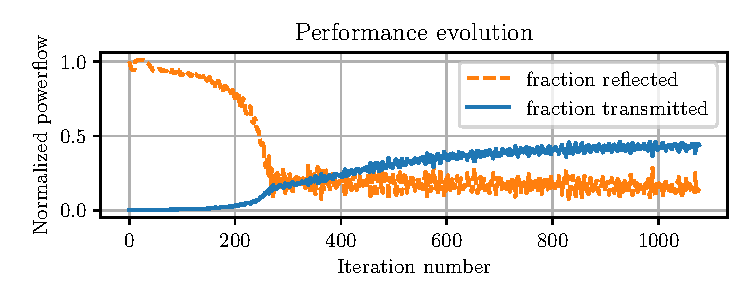
\includegraphics{chapters/results/conv_tmp.pdf}
	\caption{Still running simulation :D}%
	\label{fig:bin_conv}
\end{figure}

\begin{figure}[htpb]
	\centering
	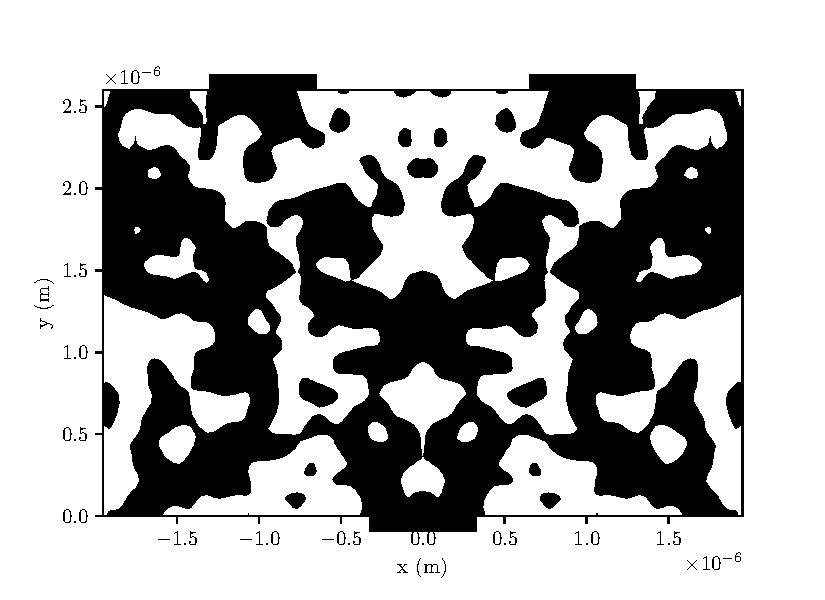
\includegraphics{chapters/results/bin_design_tmp_254.pdf}
	\caption{%
		The current best design from the level-set simulations (but they are
		still running:)
	}%
	\label{fig:bin_design}
\end{figure}
